\section{Current effects on waves: propagation}
\subsection{A uniform current}
For waves over a flat bottom, in the absence of any friction, the shape of waves and their 
motion is unchaged by a Eulerian uniform horizontal current $\Ub$. This is easily seen by changing 
the reference frame to a reference frame in which the current is zero. This is obtained with  a position $\xb'$ defined as
\begin{equation}
\xb' =\xb + \Ub t.
\end{equation} 
In particular the phase in the moving reference frame is given by eq (\ref{eq:phasecur}), and it is transformed back to the fixed reference 
frame as 
\begin{equation}
 \Theta'={\mathbf
k}\bcdot{\mathbf x} - {\mathbf
k}\bcdot \Ub t -\sigma t+ \Theta_0,  =  {\mathbf
k}\bcdot{\mathbf x} - \omega  t+ \Theta_0\label{eq:phasecur}
\end{equation}
where we have defined the absolute radian frequency, 
\begin{eqnarray}
\omega &=& \sigma + \kb \bcdot \Ub.
\end{eqnarray}

The effect of a uniform current is thus a simple Doppler shift of the phase, which gives a modification of the 
phase speed and group speed, 
\begin{eqnarray}
\Cb'&=&\Cb + \Ub \\
\Cb_g'&=&\Cb_g + \Ub,
\end{eqnarray}
where $\Cb'$ and $\Cb_g'$ are the phase and group speed in the fixed reference frame. 
$\sigma$ is called the relative radian frequency. We note that the general definition of the 
group speed still holds, 
$\Cb_g'=(\partial \omega / \partial k_x, \partial \omega / \partial k_y)$.

\subsection{Effect of current changes along the propagation direction}\label{section:bunching}
Taking a stationary current  $U(x)$ in the direction of progation $x$, or in the opposite direction, varying only in this same direction, 
the waves kinematics must adjust to this variation in current speed. 
For slow variations on the scale of the wavelength, we use the approximation by Wentzel, Kramers,
Brillouin et Jeffreys (WKBJ), i.e. the waves are locally sinusoidal, and the conservation of the number of crests (which holds for linear monochromatic waves), and which gives a constant absolute frequency $\omega$ because the medium in which the 
waves propagate is constant (an interesting case where $\omega$ is not conserved is when the water depth changes in time). 
As a result the intrinsic frequency $\sigma$ must adjust. If the current accelerates in the direction of propagation, then $\sigma$ must be 
reduced because $\kb \bcdot \Ub$ is positive. Because 
 $\sigma$ grows with $k$, the wavelength increases.
Conversely, for waves propagating against an accelerating current, $\kb \bcdot
\Ub$ is negative, hence $\sigma$ and $k$ must increases to keep $\omega$ constant.

A first application can be done in the case of deep water waves with a known 
radian frequency $\sigma_1$, propagating from a region 1
without current, to a region 2 where a current of magnitude $U$ is uniform and opposite to the waves. 

For linear waves, the number of crests is conserved, which can be written as a conservation 
of the absolute frequency,
\begin{equation}
 \sigma_2 - k_2 U = \sigma_1.
\end{equation}

Combined with the dispersion relation $\sigma_1^2 = g k_1$ and $\sigma_2^2 = g k_2$, this gives us 
a second order equation for the unknown relative frequency $\sigma_2$, 
\begin{equation}
 \frac{U}{g} \sigma_2^2 -\sigma_2 + \sigma_1 = 0.
\end{equation}
This second-order polynomial equation has two solutions, but we shall only consider the one that gives 
$\sigma_1 = \sigma_2$ when $U$ goes to zero, 
\begin{equation}
 \sigma_2 =  \sigma_1 \frac{1 - \sqrt{1-4\alpha}}{2 \alpha }
\end{equation}
with $\alpha =  U \sigma_1 / g$, the ratio of the current velocity and the phase speed $C_1=g/\sigma_1$ in region 1.
We note that there is no real solution for $\alpha < 0.25$, in that situation the waves are blocked by the current 
and cannot propagate in region 2. In the limiting case, $\alpha = 0.25$, we have $\sigma_2 = 2 \sigma_1$ and the 
local group speed $C_{g2}$ is equal to $U$. In that case there is no wave energy flux, because the 
mean wave energy velocity is $C_g-U=0$. 

We can further investigate the case when $\alpha \ll 1$. In that case, we may write the following expansion, 
\begin{equation}
 \sqrt{1-4\alpha}= 1 - 2 \alpha - 2 \alpha^2 + O(\alpha^3) 
\end{equation}
which gives 
\begin{eqnarray}
 \sigma_2 &\simeq & \sigma_1 (1+\alpha),\\
k_2 &=&  k_1 (1+2\alpha).
\end{eqnarray}
This means that the intrinsic wave period $\sigma$ is shortened in proportion to the ratio $\alpha = U/C_1$ and the wavelength 
is shortened by twice that amount. 

In  order to know what happens to the wave height, we may consider the energy balance, as we shall do later. 
But be careful, this situation is precisely a situation where the wave energy is not conserved, even without any dissipation. 
What is conserved is the total energy in the system (waves + current), and in practice the waves and currents 
exchange energy. In the absence of dissipation, this interaction happens with the conservation of another quantity, 
the wave action, which we may define for monochromatic waves as  
\begin{equation}
 A=\frac{g E}{\sigma}.
\end{equation}

With a properly defined control volume, the equality of the action fluxes gives, 
\begin{equation}
\frac{E_2}{\sigma_2}\left(C_{g2} -U\right)=\frac{E_1}{\sigma_1}C_{g1}.
\end{equation}
which gives an amplification  of the wave energy 
\begin{equation}
E_2 = E_1 \frac{\sigma_2}{\sigma_1}\frac{C_{g1}}{C_{g2} -U} \simeq E_1 (1+4 \alpha + O(\alpha^2) )
\end{equation}
in which three factors are important: 
\begin{itemize}
 \item the increase of $\sigma$ makes it necessary to increase $E$ to keep $A$ constant, 
this amplification comes with a transfer of energy from the current to the waves, this gives the factor 
${\sigma_2}/{\sigma_1} \simeq (1+\alpha)$. 

 \item the fact that the advection velocity involves the current, $C_g$ is replaced by $C_g -U$, this accounts 
for half of the total effect because $U/C_g=2 \alpha$. 
 \item the fact that the intrinsic group speed has been reduced because the wave have become 
shorter. 
\end{itemize}
As a result, the change of wave height is only proportional to $(1+2 \alpha)$, and the change in wave stepness is proportional to  $(1+4 \alpha)$. The effect of currents can be much larger for time-varying currents \citep{Ardhuin&al.2012,Peureux&al.2021}. 
 In practice, another effect can have large impacts on wave heights: refraction. 

\subsection{Effects of current gradients in the transverse direction:\\
rays and refraction}
Just like changes in water depth discussed in chapter \ref{ch5}, currents induce a modification of the phase speed. 
As a result, any current gradient in the direction transverse to the wave propagation 
will cause refraction, namely a gradual turning of the wave crests. 
The particularity of cases with current is that the direction of the phase advection 
can be different from the direction perpendicular to the crests. The directions in which rays bend follows Fermat's principle, namely waves 
will always take the path that gives the shortest propagation time. As a result, waves will focus in a jet  that flows in the direction 
opposite to the wave propagation direction (as shown in Figure \ref{fig:PN_ref}) 
and diverge in a jet of same direction.


The equations of wave rays are the trajectories followed by wave packets in time, these are identical to the propagation equations, before discretization,  
that are solved by spectral models like WAVEWATCH III \citep[equations 2.9 to 2.11 in][]{Tolman&al.2014}
\begin{equation}
\frac{{\mathrm d} \xb}{{\mathrm d} t} = {\bf C}_g + \widehat{\ub} \: , \label{eq:x_dot}
\end{equation}
\begin{equation}
\frac{{\mathrm d} k}{{\mathrm d} t} = - \frac{\partial \sigma}{\partial D}
\frac{\partial D}{\partial s} - {{\mathbf k}} \cdot
\frac{\partial \widehat{\ub}}{\partial s} \: , \label{eq:k_dot}
\end{equation}
\begin{equation}
\frac{{\mathrm d} \theta}{{\mathrm d} t} = - \frac{1}{k} \left [
\frac{\partial \sigma}{\partial D} \frac{\partial D}{\partial m}
- {{\mathbf k}} \cdot \frac{\partial \widehat{\ub}}{\partial m}
\right ] \: , \label{eq:theta_dot}
\end{equation}
where $\bf x$ is the horizontal position along the ray, $D$ is the water depth, $\theta$ is the local intrinsic wave direction, 
 ${\bf C}_g$ is the vector intrinsic group speed, pointing in direction ${\theta}$, $s$ is a coordinate in the
direction\footnote{Due to the presence of the current, $s$ differs 
from the along-ray direction.} $\theta$ and $m$ is a coordinate perpendicular to $s$. 
  These ray equations are the same as those used 
 by \cite{Mathisen1987}, with the addition of finite depth and bottom refraction effects. 

\cite{Landau&Lifschitz1960} gave a simple result on the curvature of the rays followed by wave groups in a medium with varying mean flow velocity. 
This was re-derived by  \cite{Dysthe2001} for surface gravity waves. In the limit of a weak current, $\widehat{u} \ll C$, the radius of curvature 
of the rays is 
\begin{equation}
    R=\frac{1}{\partial \theta /\partial s}= \frac{C_g}{\bnabla \times \widehat{\mathbf
    u}}
\end{equation}
where $\bnabla \times \widehat{\mathbf
    u}$ is the vertical vorticity of the flow. %This result was  applied by \cite{Gallet&Young2014} to explain the deviation, of the order of $10^\circ$,  
As the wave directions are changed, the energy of the wave can be focused by opposing current jets, %of remote swells recorded off the southern California coast, and 
explaining the occurence of very large waves in the Agulhas current \citep{Lavrenov1986}. 

%%%%%%%%%%%%%%%%%%%%%%%%%%%%%%%%%%%%%%%%%%%%%%%%%%%%%%%%%%%%%%%%%%%%%%%%%%%%%
\begin{figure}[htb]
\centerline{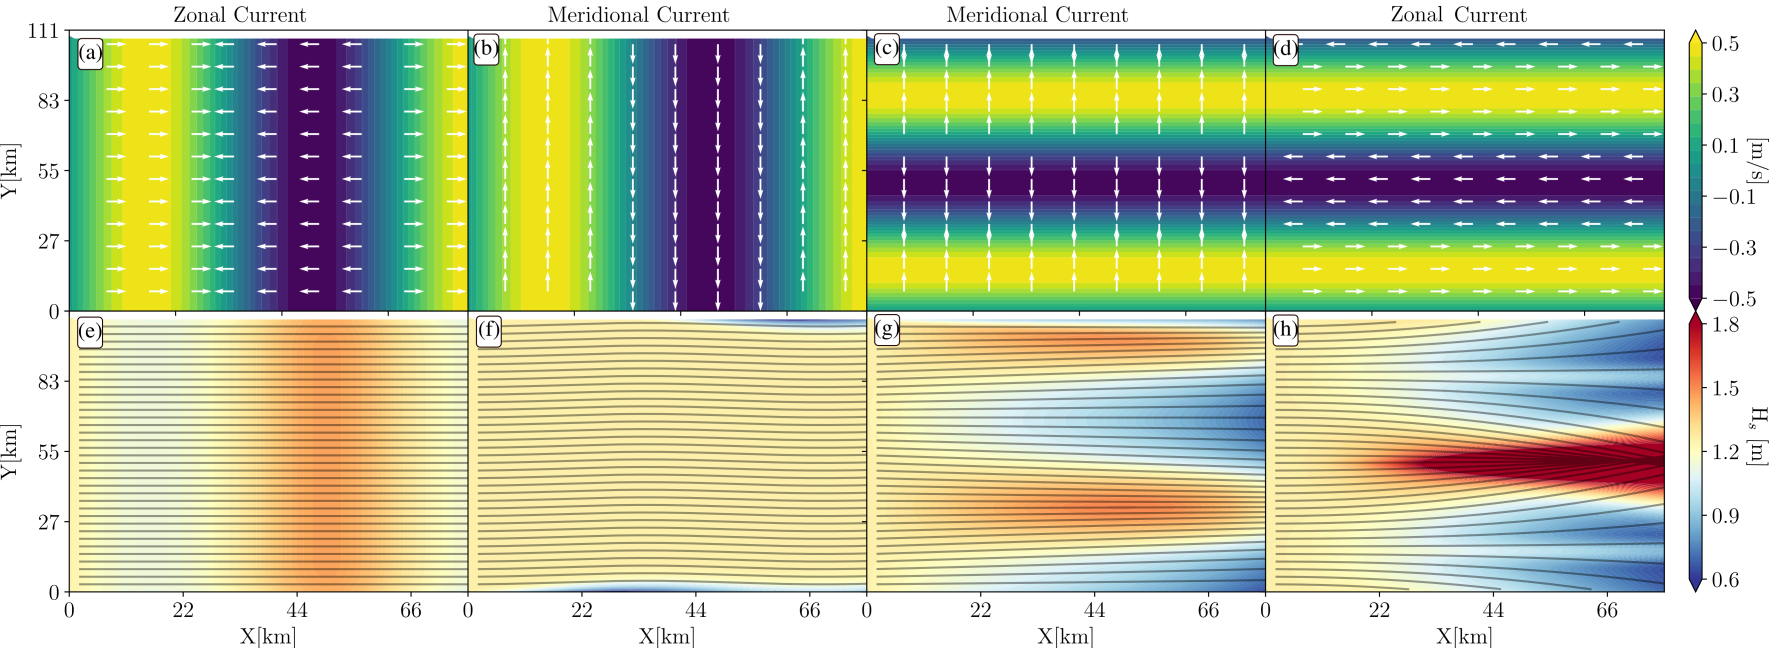
\includegraphics[width=\textwidth]{FIGS_CH_CURRENT/cosine_current.png}}
%\vspace{3.64in}
  \caption{Influence of the 4 different components of the current gradient $U \sin (K x)$, $V \sin (K x)$,  $V \sin (K y)$, $U \sin (K y)$, on waves propagating from left to right with a narrow spectrum and a period of 7~s (figure by G. Marechal).}
\label{fig:cosinecur}
\end{figure}
%%%%%%%%%%%%%%%%%%%%%%%%%%%%%%%%%%%%%%%%%%%%%%%%%%%%%%%%%%%%%%%%%%%%%%%%%%%%%
In practice the importance of refraction on wave height depends on the current structure. Gradients that are perpendicular to the dominant wave propagation and are coherent over long distances are most effective in creating a variability in the significant wave height, as shown in Fig. \ref{fig:cosinecur}. This analysis can be generalized to any current pattern to derive a map of wave heights from the map of currents \citep{Wang&al.2023}. 

Figure \ref{fig:PN_ref} shows an example off the West coast of France where the very strong vorticity of tidal currents, 
of the order of 0.001~$s^{-1}$ is enough to bend wave rays for $T=10~s$ waves with a radius of curvature of 8.6~km.
%%%%%%%%%%%%%%%%%%%%%%%%%%%%%%%%%%%%%%%%%%%%%%%%%%%%%%%%%%%%%%%%%%%%%%%%%%%%%
\begin{figure}[htb]
\centerline{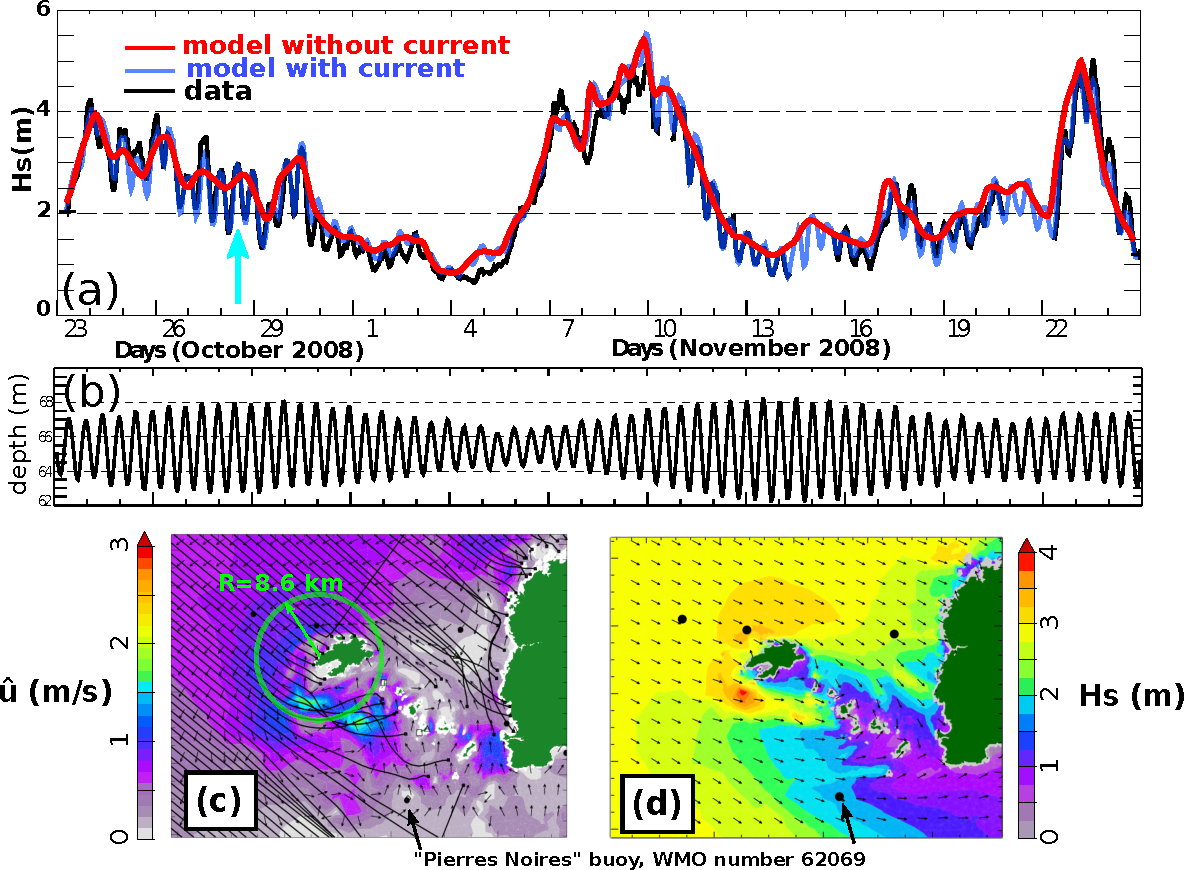
\includegraphics[width=0.95\textwidth]{FIGS_CH_CURRENT/Pierres_Noires_refraction.pdf}}
%\vspace{3.64in}
  \caption{Example of strong impact of currents on wave heights due to wave refraction by currents. The top panel shows a time series of $H_s$ 
  recorded at the wave buoy `Pierres Noires' (WMO number 62069) and modeled with WAVEWATCH III, while the middle panel shows the water depth at the buoy. The bottom 
  maps show the (c) currents provided by the numerical model MARS2D and the corresponding wave rays for $T=10$~s 
  computed by integration of eqs. (\ref{eq:x_dot})--(\ref{eq:theta_dot}), and (d) shows  $H_s$ and mean wave directions, both
  for October 28, 2008, at 11:00 AM UTC (corresponding to blue arrow in a). Clearly, the wave height has a strong 
  tidal modulation which is due to currents. The typical curvature radius of the rays is around 10~km in the current jet located south-west of the island of Ouessant. 
  This jet peaks 1.5 hours after the high tide, and deviates the waves away from the Pierres Noires buoy, 
  located 20~km down-wave \citep[Adapted from][]{Ardhuin&al.2012b}.}
\label{fig:PN_ref}
\end{figure}
%%%%%%%%%%%%%%%%%%%%%%%%%%%%%%%%%%%%%%%%%%%%%%%%%%%%%%%%%%%%%%%%%%%%%%%%%%%%%

 

\subsection{Waves over vertically sheared currents}
In the presence of vertical shear, the Laplace equation becomes the Rayleigh equation and the Doppler shift  $\kb \bcdot \Ub$ for linear waves 
can be estimated by solving it. 
\cite{Biesel1950}
gave solutions in the limit $kD \ll 1$ and for a constant shear, with a current varying from $\widehat{u}_{-D}$ at the bottom to 
$\widehat{u}_0$ at the surface. The phase speed is then 
\begin{equation}
    C=\left[\left(\frac{U_0-U_{-D}}{2}\right)^2 + gD \right]^{1/2}
\end{equation}

For more general current profiles and water depths,
\cite{Kirby&Chen1989} gave an approximate solution in the limit of small variations of $U$ compared to $\sigma/k$,
\begin{equation}
    C=\frac{\sigma}{k}+2\int_{-D}^0 {\mathbf k} \bcdot \widehat{\mathbf u} \frac{\cosh(2kz+2kD)}{\sinh(2kD)} {\mathrm d}z
\end{equation}

\subsection{Practical importance of currents}
 In practice, current effects on waves combines the `bunching' or `concertina' effect described in section \ref{section:bunching} due to a converge in the current, 
with the refraction, associated with current vorticity. A third effect is the enhancement of wave generation in waves against currents due to the relative wind. When 
we use the frame of reference moving with the current $\widehat{\mathbf u}$, the wind speed in that frame of reference changes from ${\mathbf U}_{10}$
to ${\mathbf U}_{10}-\widehat{\mathbf u}$. In practice one should thus correct the wind speed provided by a weather forecasting model to force the wind-wave generation... except 
for real adjustement of the wind to the presence of the current which are generally not included in weather models. Hence, the true wind is reduced by opposing currents
so that the wind-wave forcing should be something between the modeled ${\mathbf U}_{10}$ and ${\mathbf U}_{10}-\widehat{\mathbf u}$, say 
${\mathbf U}_{10}-r \widehat{\mathbf u}$. Numerical experiments for large scale 
currents suggests that on average $r\simeq 0.5$ is the right order of magnitude when adjusted to the fully coupled atmosphere-current 
solution (J. Bidlot, personal communication 2010). This is very important for the ocean dynamics, and forcing an ocean circulation model with $r=1$ generally gives a work of the wind against the eddies that is too strong and produces a strong underestimation of the eddy kinetic energy \citep{Renault&al.2016}, with influences on the position of western boundary currents such as the Gulf Stream \citep{Renault&al.2016b}.

In figure \ref{fig:Drake}, we show an example of modelled current effects on waves in the Drake passage, between Chile and Antarctica. 
The variability of wave heights is investigated by computed the spatial spectrum of $H_s$. We find that the 
variation in wave heights at large scales is dominated by the effect of refraction, whereas at scales around 10~km, 
the variability is mostly due to the relative wind and advection effects. Although standard processing of satellite altimeter data at scales shorter than 80~km (e.g. figure \ref{fig:Drake}.d) is dominated by noise, adaptative denoising method are now producing data that validate this strong effect of currents \citep{Quilfen&al.2018}. 

%%%%%%%%%%%%%%%%%%%%%%%%%%%%%%%%%%%%%%%%%%%%%%%%%%%%%%%%%%%%%%%%%%%%%%%%%%%%%
\begin{figure}[htb]
\centerline{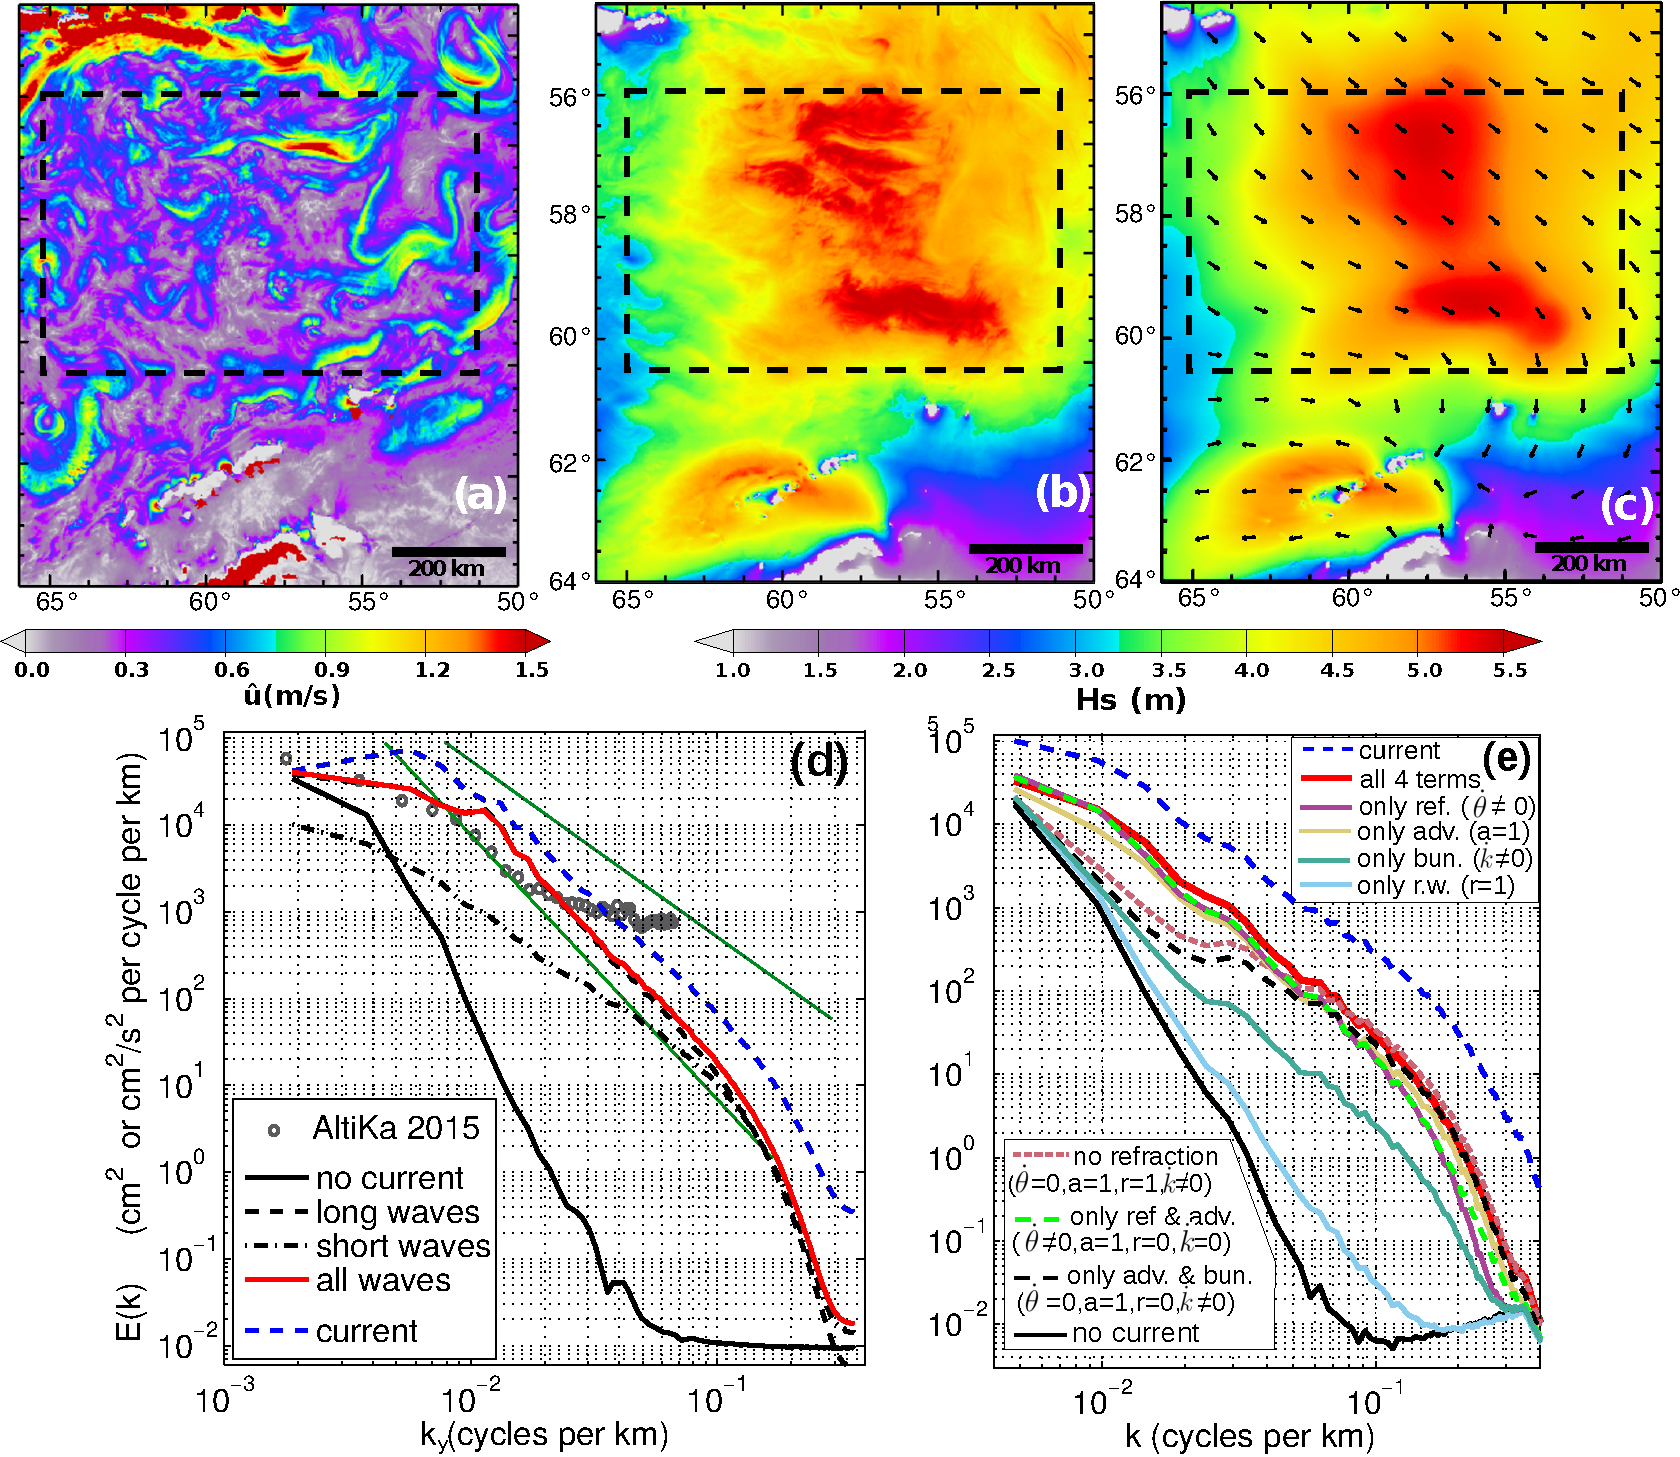
\includegraphics[width=0.8\textwidth]{FIGS_CH_CURRENT/Drake.pdf}}
%\vspace{3.64in}
  \caption{Maps for September 16 at 18:00 UTC for  (a) surface current magnitude modeled by MITgcm (b) 
the modeled significant wave height when the current forcing is included 
in WAVEWATCH III (c) significant wave height without effects of currents and wind directions (arrow). The dashed box is the region used for spectral analysis. 
(d) Spectra of the modeled zonal current and $H_s$ along the north-south direction, 
with contributions of waves of periods shorter or longer than 6~s, along-track measured spectra from AltiKa is shown for comparison, and 
power laws $k^{-2}$ and $k^{-3}$ are shown in green. (e) Omnidirectional spectrum of $H_s$ and  contributions 
of the current through the four different terms of the wave action equation (\ref{Action_balance}) can be revealed by 
progressively switching off the different terms: refraction $\dot{\theta}$, change in wavenumber $\dot{k}$, relative wind $r$, 
and advection by $u_E$ and $v_E$ in $\dot{\lambda}$ and $\dot{\phi}$. Adapted from \cite{Ardhuin&al.2017a}.
}
\label{fig:Drake}
\end{figure}
%%%%%%%%%%%%%%%%%%%%%%%%%%%%%%%%%%%%%%%%%%%%%%%%%%%%%%%%%%%%%%%%%%%%%%%%%%%%%


\section{Wave effects on currents}
To make it as simple as possible we first follow the approach of \cite{Phillips1977}, in which the velocity field  $\ub$ is the sum of a current  $\widehat{\ub}$, that we assume 
uniform over the vertical, and a perturbation $\ub'$ such that its  average is zero, at least for the points of space that are always in the water.  

\subsection{Mean flow equations integrated over the vertical}
A systematic discussion of wave effects on currents started with Longuet-Higgins and
Stewart (1964\nocite{Longuet-Higgins&Stewart1964}), and we follow their derivation. The three-component momentum vector $\rho (u,v,w)$ can be advected in any direction, 
giving a flux tensor $\rho u_i u_j$.  When one considers only velocity fluctuations $\ub'$, the momentum flux due to the self-advection of momentum 
is the usual Reynolds stress $-\rho u_i' u_j'$, which is used in the analysis of turbulence.  The divergence of this flux is equivalent to 
a macroscopic force that accelerates the fluid particles, which is easily understood by considering the momentum balance over an elementary cube. 
 
Longuet-Higgins and
Stewart (1964\nocite{Longuet-Higgins&Stewart1964}) introduced a similar tensor caused by waves, the radiation stress $S^{\mathrm{rad}}$, that is confined to the two horizontal dimensions, 
it represents a flux of 
momentum that comes from the average of the wave-induced Bernoulli pressure $p+u^2$. Compared to Taylor expansion methods, the present 
approach is easier because the non-linear wave effects are directly included by using conservation equations. 


Starting from the conservation of momentum in any horizontal direction $\alpha$, with our notation $u_\alpha$ is either the $u$ or the $v$ component, 
\footnote{Taking into account viscosity and the air pressure  $p_a$ 
allows to include the surface and bottom stress, which are not in the derivation by \cite[][page 62]{Phillips1977}.} 
\begin{equation}
 \frac{\partial }{\partial t} \left(\rho_w u_\alpha\right)+ \frac{\partial }{\partial x_\beta} 
\left(\rho_w u_\alpha u_\beta + p \delta_{\alpha \beta} \right)
+ \frac{\partial }{\partial z} \left(\rho_w u_\alpha w \right)  + \varepsilon_{\alpha \beta i} f_i \rho_w u_\beta = \rho_w \nu \frac{\partial^2 u_\alpha}{\partial z^2},\label{NavierStokes_horiz}
\end{equation}
in which there is an implicit sum over the repeated indices, here $\beta$, and where  $\varepsilon_{\alpha j i} f_i u_j$ 
is the $\alpha$  component of the vector product of the Coriolis parameter vector with the speed vector. In the following we classically 
consider only the vertical Coriolis parameter  $f_3$.

To be sure that we understand the implicit sum, an explicit form of the equation for the $u$ component is, 
\begin{equation}
 \frac{\partial }{\partial t} \left(\rho_w u\right)+ \frac{\partial }{\partial x} 
\left(\rho_w u^2  + p  \right) + \frac{\partial }{\partial y} 
\left(\rho_w uv \right)
+ \frac{\partial }{\partial z} \left(\rho_w u w \right)  - f_3 v = \rho_w \nu \frac{\partial^2 u}{\partial z^2},\label{NavierStokes_horiz_exp}
\end{equation}

Integrating over the vertical, and using the boundary conditon at the surface and bottom, 
$w(\zeta)=\partial \zeta/\partial t + \ub \bcdot \bnabla \zeta$, yields 
\begin{eqnarray}
 \frac{\partial }{\partial t} \int_{-h}^{\zeta} \rho_w u_\alpha \mathrm{d} z 
&+ &\frac{\partial }{\partial x_\beta}\int_{-h}^{\zeta}  \left(\rho_w u_\alpha u_\beta  + 
\delta_{\alpha \beta} p\right)   \mathrm{d} z +
\varepsilon_{\alpha \beta 3} f_3 \int_{-h}^{\zeta} \rho_w u_\beta \mathrm{d} z  \nonumber \\
&=&p_a \frac{\partial \zeta}{\partial x_\alpha} - p(-d)\frac{\partial h}{\partial x_\alpha}  + \rho_w \nu \frac{\partial u_\alpha}{\partial z}|_{z=\zeta} - \rho_w \nu \frac{\partial u_\alpha}{\partial z}|_{z=-h} \label{Phillips1}
\end{eqnarray}

We now take the average over wave phases \footnote{\cite{Phillips1977} uses a horizontal average 
but as a result the obtained equatiosn are only valid at scales larger than the wavelength. Using the phase average allows to keep 
sub-wavelength variations such as in the case of partial standing waves, see \cite{Ardhuin&al.2008}.}. 

The second integral in \ref{Phillips1}, gives, on average\footnote{This is here that we use the fact that  $\hu$ is independent of  
$z$, otherwise we would have an extra term coming from the vertical current profile, 
that would be equivalent to a horizontal mixing term \citep{Svendsen&Putrevu1994}.}, using  $u=\hu+u'$, 
\begin{eqnarray}
\overline{ \int_{-h}^{\zeta}   \rho_w u_\alpha u_\beta \mathrm{d} z } &= & \rho_w  \int_{-h}^{\overline{\zeta}} \hu_\alpha \hu_\beta   \mathrm{d} z
 +   \rho_w \hu_\alpha \overline{ \int_{0}^{\zeta} u'_\beta \mathrm{d} z } + \rho_w \hu_\beta \overline{ \int_{0}^{\zeta} u'_\alpha \mathrm{d} z }
 + \overline{ \int_{-h}^{\zeta} \rho_w u'_\alpha u'_\beta 
\mathrm{d} z}.\label{eq:ch7:advection}
\end{eqnarray}
We now define the $\alpha$-component of the total mass transport vector as\footnote{This notation 
differs from \cite{Phillips1977} who used $\widetilde{M}_\alpha$.}, 
\begin{equation}
M_\alpha = \overline{ \int_{-h}^{\zeta}   \rho_w u_\alpha \mathrm{d} z } 
\end{equation}
and the wave-induced mass transport, also known as the Stokes transport\footnote{The decomposition \ref{Phillips_advection} 
and this definition of the Stokes transport require, to be well defined, an analytical extension of the velocity field  $u'$ in the air. 
This is not the real velocity field which, like the density, is very different from this extension. A nice way to avoid this issue is to use an average
that follows the up-and-down motion of the sea surface \citep[e.g.][]{Ardhuin&al.2008b}.}, 
and the difference of these two is the mass transport due to the mean flow
\begin{equation}
M_\alpha^m = M_\alpha - M_\alpha^w = \overline{ \int_{-h}^{\zeta}   \rho_w \hu_\alpha \mathrm{d} z } =\hu_\alpha  \overline{ \int_{-h}^{\zeta}   \rho_w \hu_\alpha \mathrm{d} z} = \rho_w D \hu_\alpha.
\end{equation}
We can thus re-write  eq. (\ref{eq:ch7:advection}) as 
\begin{eqnarray}
\overline{ \int_{-h}^{\zeta}   \rho_w u_\alpha u_\beta \mathrm{d} z }   & = & \frac{1}{\rho_w D} \left(M_\alpha^m M_\beta^m + M_\alpha^m M_\beta^w  + M_\beta^m M_\alpha^w\right) + \overline{ \int_{-h}^{\zeta} \rho_w u'_\alpha u'_\beta 
+\delta_{\alpha,\beta}} p\mathrm{d} z  \\
& = & \frac{1}{\rho_w D} \left(M_\alpha M_\beta - M_\beta^w M_\alpha^w\right) + \overline{ \int_{-h}^{\zeta} \rho_w u'_\alpha u'_\beta 
\mathrm{d} z}. \label{Phillips_advection}
\end{eqnarray}

The conservation of the vertical momentum is, neglecting viscosity and turbulence, 
\begin{equation}
 \frac{\partial }{\partial t} \left(\rho_w w\right)+ \frac{\partial }{\partial x} 
\left(\rho_w u w   + p  \right) + \frac{\partial }{\partial y} 
\left(\rho_w v w   + p  \right)+ \frac{\partial }{\partial z} \left(\rho_w w^2 \right)   = - \rho_w g.
\end{equation}
A vertical integration gives, after using the surface kinematic boundary condition, 
\begin{equation}
 p(z)=p_a + g\int_{z}^{\zeta} \rho_w \mathrm{d}z + \frac{\partial }{\partial t} \int_{z}^{\zeta} \rho_w w  \mathrm{d}z  
+ \frac{\partial }{\partial x_\beta} \int_{z}^{\zeta} \rho_w  u_\beta w  \mathrm{d}z
- \rho_w w^2(z).\label{p_z}
\end{equation}
in which the second term is the hydrostatic pressure, and the third
vanishes only if the spatial average is independant of time -- which is not the case in the presence of waves travelling in opposite directions as shown in chapter \ref{chsismo} --  
the fourth term vanishes for a motion that is periodic in time, and the 
last term is the mean dynamic pressure which is zero only if the velocity is zero.  If we make all these assumptions 
the bottom pressure is hydrostatic, 
\begin{equation}
 p(-h)=\rho_w g D + p'.
\end{equation}
As a result the mean value of the right hand side of (\ref{Phillips1}) is 
\begin{equation}
\tau_{a,\alpha} - \tau_{b,\alpha} + \rho_w g D \frac{\partial h}{\partial x_\alpha}= \tau_{a,\alpha} - \tau_{b,\alpha} + \frac{\partial }{\partial x_\alpha}\left(\frac{1}{2} \rho_w g D^2 \right)
-\rho_w g D \frac{\partial \overline{\zeta}}{\partial x_\alpha},
\end{equation}
where $\tau_{a,\alpha}$  and $\tau_{b,\alpha}$ are the $\alpha$-components of the surface and bottom stress. 
The correlation $p' \partial h/ \partial x_\alpha$ has been included in $\tau_{b,\alpha}$ as it represents the form drag 
on the bottom, while the other part of $\tau_{b,\alpha}$ is the skin friction given by the average of the viscous stress. 

We now have \citep{Smith2006b}, 
\begin{equation}
\fbox{$\displaystyle \frac{\partial M_\alpha }{\partial t} + \frac{\partial }{\partial x_\beta} \left( \frac{M_\alpha M_\beta-M_\alpha^w M_\beta^w}{\rho_w D} 
+ S^{\mathrm{rad}}_{\alpha \beta}\right) +\varepsilon_{\alpha \beta 3} f_3 M_\beta  = -\rho_w g D \frac{\partial \overline{\zeta}}{\partial x_\alpha} + \tau_{a,\alpha} - \tau_{b,\alpha}.$}\label{Phillips_mom}
\end{equation}
where the radiation stresses are defined by \cite{Phillips1977} as the difference between the momentum flux and the flux in the absence of waves, 
\begin{equation}
    S^{\mathrm{rad}}_{\alpha \beta}=\overline{\int_{-h}^\zeta \rho_w u_\alpha u_\beta +\delta_{\alpha \beta}  p \mathrm{d}z }
    -\frac{1}{2} \rho_w g D^2 \delta_{\alpha \beta}  - \rho_w \hu_\alpha \hu_\beta D. \label{Srad_def_Phillips}
\end{equation}
The expression for $S^{\mathrm{rad}}$ using linear wave theory is given in chapter \ref{ch_momentum}.

The same procedure applied to the mass conservation equation yields 
\begin{equation}
\fbox{$\displaystyle \frac{\partial M_\beta }{\partial x_\beta} + \rho_w \frac{\partial D}{\partial t}=0.$}\label{Phillips_mass}
\end{equation}

Equations (\ref{Phillips_mom}) and (\ref{Phillips_mass}) are the basic equations used in nearshore hydrodynamics, in their most 
simple form. They can be used to explain a wide variety of phenomena, from changes in the mean sea level, along-shore currents in the 
surf zone, infra-gravity waves ....  All these will be discussed in chapter \ref{ch_littoral}. The assumptions made by 
 \cite{Phillips1977} are fairly restrictive. Removing many of these, we present in chapter \ref{ch_vaguescourant3D} an extenstion of the wave-current interaction theory to three dimensions. 

We note that the mass transport $M_\alpha$ can be expressed with a mean velocity $U_\alpha$ ad $M_\alpha=\rho_w D U_\alpha$. 
This mean velocity includes the Stokes drift, which usually has a strong vertical gradient, even possibly in the surf zone  \citep{Ardhuin&al.2008}
and the mean current which can also have a strong vertical shear. 
This mean speed can thus be very different from a measured mean velocity (Eulerian mean), 
and also different from a tracer mean speed if tracers are not homogeneously 
distributed over the vertical, as it is the case for suspended sediment. 




\subsection{Total energy}
From the momentum equation the energy equation can be derived. With a viscous dissipation rate $\epsilon$ per unit volume and the stress 
tensor $p \delta_{ij} + \tau_{ij}$,  in which $i$ and $j$ can be any of the three directions  $x$, $y$ and $z$, 
\begin{equation}
 \frac{\partial }{\partial t}\left(\rho_w \frac{u_i u_i }{2}   + g z\right) + \frac{\partial }{\partial x_j}
 \left[u_i \left( \rho_w \frac{u_i u_j }{2}   + g z + \delta_{ij} p + \tau_{ij} \right) \right] 
= \epsilon.\label{emeca_local}
\end{equation}


Following the derivation of \citet[][page 63]{Phillips1977}, and defining the total depth-integrated mechanical energy per unit surface as
\begin{equation}
 E_a = \overline{\int_{-h}^\zeta \rho_w \left(\frac{1}{2} u_i u_i + gz\right)  \mathrm{d}z} = \frac{1}{2} \frac{M_\alpha M_\alpha}{\rho_w D} + 
 \hu_\alpha M^w_\alpha + \frac{1}{2} \rho_w g (\overline{\zeta}^2 - h^2) - \frac{1}{2} \rho_w \hu_\alpha \hu_\alpha + \rho_w g E + E', 
\end{equation}
in which $\rho_w g E$ is the wave energy per unit surface and $E'$ is the turbulent energy.

Integrating (\ref{emeca_local}) over depth and using eq. (\ref{Srad_def_Phillips}) for $S^{\mathrm{rad}}$, we get  
\begin{eqnarray}
 \frac{\partial E_a}{\partial t} & + & \frac{\partial }{\partial x_\alpha} \left( U_\alpha E_a + F_\alpha + 
\rho  U_\alpha g h^2 + \hu_\beta S^{\mathrm{rad}}_{\alpha \beta} \right) \nonumber \\
&=& - \overline{\left[ w  p + \tau_{i 3} u_i \right]^{\zeta}_{-h}}+ \overline{ \left( u_\alpha  p
 + \tau_{i \alpha} u_i \right)\frac{\partial \zeta}{\partial x_\alpha}}+ \overline{\int \epsilon {\mathrm d}z}, \label{E_a}
\end{eqnarray}
in which the energy flux $F_\alpha$ is 
\begin{equation}
 F_\alpha =  \overline{\int_{-h}^\zeta u_\alpha \left[ \frac{1}{2}  \rho_w  u_i'^2 +  \rho_w  g(z-h)+ p + \tau_i \alpha \right]  \mathrm{d}z}.
\end{equation}

\section{Energy exchange and wave action}
We can then subtract the mean flow energy $\left[ U_\alpha \times \right.$ (\ref{Phillips_mom})$+ (gh - U_\alpha^2/2 )\times $(\ref{Phillips_mass})$\left.\right]$ 
from (\ref{E_a}) to obtain the wave energy evolution equation\footnote{Here it is assumed that  $\hu$ is a vertically-uniform current. 
In a more general case $\hu$ is replaced by $u_A$ as defined by eq.  
(\ref{dispersionD3}). There are still discussions about the interpretation of this, but it was derived by \cite{Andrews&McIntyre1978b}.}, 
\begin{equation}
 \rho_w g \frac{\partial E}{\partial t}+ \frac{\partial }{\partial x_\alpha}\left[\rho_w g E \left(\hu_\alpha + C_{g \alpha}\right)\right]
+  S^{\mathrm{rad}}_{\alpha \beta} \frac{\partial \hu_\beta}{\partial x_\alpha}  = \phi_{aw} - \phi_{oc} - \phi_{bf},\label{ewave}
\end{equation}
where $\phi_{aw}=- \overline{\left. w  p + \tau'_{i 3} u'_i \right|_{z=\zeta}}$ is the mean wind to wave energy flux per unit surface, 
$\phi_{oc}$ is the part of $-\epsilon$ associated to wave breaking and dissipation in the water column, and 
$\phi_{bf}$ is the wave energy lost through bottom friction, which will be further discussed in  chapter \ref{ch_wbbl}.

The term of particular interest to us is the gain or loss of wave energy  $S^{\mathrm{rad}}_{\alpha \beta} {\partial \hu_\beta}/{\partial x_\alpha}$,
when they propagate through current gradients, even without dissipative processes. This is indeed an exchange of energy between waves and currents. 

To simplify this term, one can introduce the wave action $A=\rho_w g E/\sigma$ \citep{Bretherton&Garrett1968,Andrews&McIntyre1978b}, and using 
the evolution equation for the wave number, we obtain \citep[see][for details]{Phillips1977}
\begin{equation}
\frac{\partial A}{\partial t}+ \frac{\partial }{\partial x_\alpha}\left[A\left(\hu_\alpha + C_{g \alpha}\right)\right]
   = \frac{\phi_{aw} - \phi_{oc} - \phi_{bf}}{\sigma}.\label{awave}
\end{equation}

The action like the energy and the momentum is a quadratic quantity. It can be decomposed into a spectrum $N\left(k,\theta,\phi,\lambda,t\right)=E\left(k,\theta,\phi,\lambda,t\right)/\sigma$ 
where  $\phi$ and $\lambda$ define the horizontal position, here the longitude and latitude. The spectral wave action equation is \citep{WAMBook}
\begin{equation}
    \frac{\partial }{\partial t}N
    +\frac{\partial }{\partial \phi}\left(\dot{\phi} N\right)
    +\frac{\partial }{\partial \lambda}\left(\dot{\lambda} N\right)
    +\frac{\partial }{\partial k}\left(\dot{k} N\right)
    +\frac{\partial }{\partial \theta}\left(\dot{\theta} N\right)
    =\frac{S}{\sigma},\label{Action_balance}
\end{equation}
where $S$ is the sum of the source terms that represent the interactions with winds, bottom, wave-wave interactions and dissipation, and
 $\theta$ is the wave propagation azimuth, the angle between North and the wave propagation direction. The propagation speeds in physical and 
spectral space are given by \cite{Tolman1990b},
\begin{eqnarray}
\dot{\phi} & = & \left(C_g \cos \theta + \hv \right) R^{-1} \\
\dot{\lambda} & =
    & \left(C_g \sin \theta + \hu \right) \left(R \cos \phi\right)^{-1} \\
\dot{\theta} & = & C_g \sin \theta \tan \phi R^{-1} 
    +\sin\theta\frac{\partial \omega}{\partial \phi}
    -\frac{\cos \theta}{\cos \phi}\frac{\partial \omega}{\partial \lambda}
    \left(kR\right)^{-1}\\
\dot{k} & = &-\frac{\partial \sigma}{\partial D} \frac{\kb}{k} \bcdot \bnabla D - \kb \bcdot  \bnabla\widehat{\mathbf{u}},
\end{eqnarray}
where $R$ is the radius of the Earth, $\hu$ and $\hv$ are the zonal (towards the East) and meridional (towards the North) components of the horizontal current $\widehat{\mathbf{u}}$.

In the absence of dissipative processes,  $S=0$ and the wave action is conserved. This is a general physical result 
and the action is an adiabatic invariant. It is the same for a pendulum of varying length,  $A=E/\sigma$ is conserved, not $E$. 
More exactly, the total wave action, integral of $A(k,\theta)$ over the spectrum, is conserved
for adiabatic processes that are independent of the wave phases. This is Noether's theorem. % Wave action is thus conserved by  4-wave interactions discussed but it is not conserved with shallow-water 3-wave interactions. In the context of wave-particle equivalence, $A$ is equivalent to the number of particles. 

As we have seen above in section \ref{section:bunching}, the conservation of wave action can be used to investigate the amplification of waves 
across a current convergence.



